
\documentclass[a4paper,11pt]{article}
\usepackage[utf8]{inputenc}
\usepackage[top=1.8cm,bottom=2.0cm,right=1.35cm,left=1.35cm]{geometry}
\usepackage{url}
\usepackage[natbibapa]{apacite}
\bibliographystyle{apacite}
\usepackage{graphicx}
\usepackage{amsmath}
\usepackage{amsfonts}
\usepackage{amssymb}
\usepackage[onehalfspacing]{setspace}
\usepackage{enumitem}
\usepackage{hyperref}
\usepackage{listings}
\usepackage{color}

\usepackage{lipsum}% this generates fictitious text for sample
%opening
\title{Twitter Dataset Analysis\\ Group 17}
\author{
    \begin{tabular}{lll}
    \textbf{Name} & \textbf{Student Number (SN)} & \textbf{Contribution} \\
    Karan Goel & 7836685 & 14.28\% \\
    Alvin Jose & 8066358 & 14.28\% \\
    Ashutosh Bhosale & 7795786 & 14.28\% \\
    Banin Sensha Shreshta & 8447196 & 14.28\% \\
    Gaurav Adarsh Santosh & 7032663 & 14.28\% \\
    Lino Thankachan & 7926017 & 14.28\% \\
    Rishab Manokaran & 7863974 & 14.28\% \\
    \end{tabular}
}


\date{CSCI946 Big Data Analytics Assignment 2\\
September 20, 2024}

\begin{document}
\maketitle
\newpage
\section{Introduction}

In this assignment, the primary objective is to detect misinformation on social networks by identifying profiles that are incorrectly classified as human or non-human. The focus of the analysis will be on the Twitter user dataset, where we aim to explore methods to distinguish between genuine and artificially generated accounts. To achieve this, we will follow a structured approach outlined in Tasks 1-4.

Task 1 involves designing a comprehensive big data analytics project, adhering to the principles of the Big Data Analytics Lifecycle.

In Task 2, the dataset will be processed by taking into account the various data types and properties. Core models and algorithms will be applied, including regression, association rules, clustering, classification, and text processing methods.

Task 3 focuses on visualizing the dataset and utilizing visual representations to evaluate the analysis results. This step will provide valuable insights into the data and help validate the findings.

Finally, Task 4 entails a detailed study of various profile factors, such as text, color, and tweet content. Based on this analysis, recommendations will be made to adjust the classification of human and non-human profiles.

\section{Task 1: Data Analysis Design}

\subsection{Learn Business Domain}
\textbf{Objective}: The aim of assignment this is to identify profiles on social networks that are mistakenly recorded as human or non-human profiles (e.g., bots).\\
\textbf{Specific Task}: You need to identify if the user’s gender is either human (male, female) or non-human(brand) based on their Twitter profile data and associated tweets.\\
\textbf{Dataset}: The dataset for this classification task can be accessed via Kaggle at the \href{https://www.kaggle.com/datasets/crowdflower/twitter-user-gender-classification}{Twitter User Gender Classification dataset}.

\subsection{Define Resources \& Goals}
\textbf{Data Source}: Twitter user profiles including tweets, descriptions, link color, sidebar color, and other metadata.\\
\textbf{Primary Task}: Classify gender into two categories: human or non-human.\\
\textbf{Key Questions}:
\begin{itemize}
    \item How well do the words in tweets and profiles predict the user as human or non-human?
    \item What are the specific words that strongly predict human or non-human?
    \item How well do other factors (like link color, tweet count, retweet count, favourite number) predict user as human or non-human?
\end{itemize}

\subsection{Frame the Problem \& Develop Initial Hypotheses}
\textbf{Problem Type}: This is a supervised learning problem where the task is to predict a categorical variable (gender: male, female, or brand).\\
\textbf{Hypotheses}:
\begin{itemize}
    \item \textbf{Null Hypothesis (H0)}: Words in tweets and profiles do not have a significant effect on predicting user as human or non-human (i.e., the predictive power is random or weak).
    \item \textbf{Alternative Hypothesis (H1)}: Words in tweets and profiles have a significant effect on predicting user as human or non-human (i.e., they provide strong predictive power).
    \item \textbf{Additional Hypotheses}:
    \begin{itemize}
        \item \textbf{H0}: Other factors (link color, tweet count, retweet count, favourite number) are not good predictors of human or non-human.
        \item \textbf{H1}: Other factors can strongly predict of human or non-human.
    \end{itemize}
\end{itemize}

\subsection{Data Preparation}
\textbf{Preprocessing Steps}:
\begin{itemize}
    \item \textbf{Stemming \& Lemmatization}: To reduce words to their base or root forms.
    \item \textbf{Lowercasing}: To eliminate discrepancies between uppercase and lowercase letters.
    \item \textbf{Tokenization}: Split text into individual words or tokens.
    \item \textbf{Embedding}: Use word embeddings (e.g., Word2Vec, GloVe, or TF-IDF) to represent text data numerically.
    \item \textbf{Bag of Words}: A simple and effective method for text representation.
    \item \textbf{Word2Vec}: A simple model to generate world embeddings.
\end{itemize}

\subsection{Visualize Data}
\textbf{Visualization Techniques}:
\begin{itemize}
    \item \textbf{Word Cloud}: To display frequent words by gender category (male/female/brand).
    \item \textbf{Word Distance/Similarity}: Use techniques like cosine similarity to understand which words or phrases are closer to each gender category.
\end{itemize}

\subsection{Model Building}
\textbf{Classification Models}:
\begin{itemize}
    \item \textbf{K-Nearest Neighbors (KNN)}, \textbf{Support Vector Machines (SVM)}, \textbf{Decision Trees}, \textbf{Random Forest}.
\end{itemize}
\textbf{Clustering Models}:
\begin{itemize}
    \item \textbf{K-Means}, \textbf{DBSCAN}, \textbf{Self-Organizing Maps (SOM)}.
\end{itemize}
\textbf{Regression Models}:
\begin{itemize}
    \item \textbf{Linear Regression}, \textbf{Logistic Regression}.
\end{itemize}
\textbf{Neural Networks}:
\begin{itemize}
    \item Build deep learning models to classify gender using \textbf{Neural Networks}.
\end{itemize}

\subsection{Training and Testing}
\textbf{Cross-Validation}: Use \textbf{k-fold cross-validation} to prevent overfitting and assess model generalization.\\
\textbf{Grid Search}: Optimize hyperparameters by performing grid search to select the best model configuration.

\subsection{Deliverables}
\textbf{Evaluation Metrics}:
\begin{itemize}
    \item \textbf{Confusion Matrix}: To visualize the performance of each classification model.
    \item \textbf{Accuracy}: The percentage of correctly classified instances.
    \item \textbf{Precision}: The proportion of true positives out of all positive predictions.
    \item \textbf{Recall}: The proportion of true positives out of all actual positives.
    \item \textbf{Loss Curves}: For neural networks, to visualize the training process and detect overfitting or underfitting.
\end{itemize}


\section{Task 2: Data Processing \& Model Application}

The dataset was loaded using the \texttt{load\_data} method from the \texttt{Task1} class, which reads a CSV file containing Twitter user data. After loading, the data was preprocessed to make it suitable for the classification task.

\subsection{Data Filtering}
\begin{itemize}
    \item Rows with a \texttt{gender:confidence} score greater than 0.9 were selected to ensure data quality.
    \item The \texttt{gender} labels were restricted to three categories: \texttt{male}, \texttt{female}, and \texttt{brand}.
    \item The \texttt{gender} column was relabeled: \texttt{male} and \texttt{female} were grouped into a \texttt{human} class, while \texttt{brand} was grouped into the \texttt{non-human} class.
\end{itemize}

\subsection{Handling Missing Values}
Missing values were filled with empty strings (\texttt{''}) to avoid issues during text processing and model training.

\subsection{Feature Selection}
The key features selected for the classification task were \texttt{gender}, \texttt{fav\_number}, \texttt{retweet\_count}, \texttt{tweet\_count}, and \texttt{text}.

\subsection{Feature Scaling and Label Encoding}
Two important steps were applied to further process the numerical and categorical data:

\subsubsection{Scaling Features}
We used \texttt{StandardScaler} to normalize numerical features such as \texttt{fav\_number}, \texttt{retweet\_count}, and \texttt{tweet\_count}. This step ensures that all features are on a similar scale, improving the performance of machine learning algorithms.

\subsubsection{Label Encoding}
The \texttt{gender} column was encoded using \texttt{LabelEncoder} to convert the \texttt{human} and \texttt{non-human} categories into numerical labels.

\subsection{Exploratory Data Analysis}
To better understand the relationships between features, we performed the following analyses:

\subsubsection{Correlation Matrix}
We computed the correlation matrix for the numerical features to observe the strength of linear relationships between variables. P-values were calculated for each pair of features to identify significant correlations. A heatmap was generated to visualize only significant correlations (with p-values less than 0.05). Figure \ref{fig:corr}

\subsubsection{Pairplot}
A scatterplot matrix (pairplot) was created to visualize relationships between the numerical features. This helped in detecting patterns and potential outliers in the dataset. Figure \ref{fig:p_plot}

\subsection{Text Processing}
Since the core of this classification task involves analyzing text data (tweets), we employed several text preprocessing techniques:

\subsubsection{Denoising}
The text was cleaned by removing unwanted characters such as URLs, HTML tags, punctuation, hashtags, and special characters using various utility methods such as \texttt{remove\_html}, \texttt{remove\_url}, and \texttt{remove\_punctuation}.

\subsubsection{Standardization}
All text was converted to lowercase using the \texttt{standardize\_text} method to avoid case-sensitive discrepancies.

\subsubsection{Lemmatization}
The \texttt{WordNetLemmatizer} was used to reduce words to their base forms (lemmas), making the text more uniform for the model while preserving meaning.

\subsubsection{Stopword Removal}
Common stopwords (e.g., ``and'', ``the'', ``is'') and irrelevant words like ``RT'', ``like'', and ``follow'' were removed to focus on meaningful words.

\subsubsection{Word Cloud Visualization}
A word cloud was generated to visualize the most frequent words across all tweets, providing insight into the dominant terms associated with the gender categories. Figure \ref{fig:wc}

\subsection{Feature Extraction}
To convert the processed text data into a numerical format suitable for machine learning models, we employed two feature extraction techniques:

\subsubsection{Bag of Words (BoW)}
The text data was vectorized using \texttt{CountVectorizer}, transforming the text into a sparse matrix of token counts. This simple and effective method allowed us to represent the frequency of words in each tweet. The resulting dense array was stored in the dataset as the \texttt{bow\_feature}. This Bow can be seen in added in this Figure \ref{fig:df}.

\subsubsection{Word2Vec Embeddings}
Word2Vec embeddings were computed using the \texttt{Word2Vec} model from the Gensim library. This method captured semantic information by learning distributed vector representations of words. The average embedding for each tweet was calculated and stored as \texttt{word2vec\_embeddings} in the dataset.








\section{Classification Models}

In this section, we explore various classification models applied to our dataset. The primary goal is to classify the given data into distinct categories using supervised learning techniques. We evaluate the models based on several performance metrics, such as accuracy, F1-score, recall, and confusion matrices. These metrics are particularly important for evaluating the performance of models in detecting misinformation on Twitter, where distinguishing between human and non-human profiles (bots) can have significant implications for stakeholders, such as social media platforms and marketers. 

Various methods such as regression, association rules, clustering, classification, and text processing were considered for this study. Each method has unique advantages and is suitable for different types of data and problems. Classification models were paid special attention for this task due to the need for distinguishing between bot and human profiles. Text processing methods like TF-IDF were crucial for converting the tweet content into a usable numerical form, making the combination of classification and text processing highly effective.

\subsection{Data Preprocessing}

The dataset was preprocessed by standardizing the features using a pipeline approach that ensures consistent transformations across models. Data was split into training and testing sets using a 70:30 ratio to enable model generalization on unseen data.

\subsubsection{Feature Extraction}

Textual data from tweets was cleaned by removing special characters, stopwords, and URLs. Tokenization and vectorization using Term Frequency-Inverse Document Frequency (TF-IDF) were applied to convert the text into numerical form, suitable for classification models. TF-IDF helps highlight important terms in a document relative to the entire corpus, which is critical when analyzing the content of tweets for classification (Ramos, 2003).

Profile attributes such as username, location, and profile colors were used as additional features. Missing values were imputed using mean values for continuous features and the most frequent value for categorical features. One-hot encoding was employed to transform categorical variables into numerical form, ensuring that they are usable by classification models.

\subsection{Model Selection}

Several classification models were considered, each offering unique advantages in terms of bias-variance tradeoff, interpretability, and performance on high-dimensional data. The models implemented are:

\subsubsection{K-Nearest Neighbors (KNN)}

KNN is a simple, non-parametric method used for classification. It classifies a data point based on the majority label among its nearest neighbors in the feature space. We used the Euclidean distance metric, and the optimal number of neighbors ($k$) was selected using GridSearchCV.

KNN is effective for datasets with high-dimensional features, such as Twitter profiles that include both textual and categorical variables. Its reliance on local data patterns is useful when detecting subtle distinctions between human and non-human behavior in social networks (Zaki \& Meira, 2014).

\subsubsection{Support Vector Classifier (SVC)}

Support Vector Classifier constructs a hyperplane in a high-dimensional space to separate different classes. The kernel function was set to radial basis function (RBF), and the regularization parameter (C) was tuned using cross-validation. SVC is particularly useful for datasets with complex class boundaries and sparse data, such as those found in social media networks, where it excels at handling high-dimensional feature spaces (Cortes \& Vapnik, 1995).

\subsubsection{Decision Tree Classifier}

Decision Trees split the data based on feature values to maximize information gain at each step. We experimented with different tree depths to prevent overfitting. Decision Trees are highly interpretable and work well with both categorical and numerical data, making them suitable for Twitter profile data, but they can suffer from high variance when not properly tuned (Quinlan, 1986).

\subsubsection{Random Forest Classifier}

Random Forests consist of multiple decision trees trained on different subsets of the data. This ensemble technique reduces variance by averaging the predictions of individual trees, leading to better generalization on unseen data. We tuned the number of trees and the maximum depth to optimize performance. Random Forests are particularly effective in handling noisy datasets and are capable of identifying feature importance, which is useful in understanding which aspects of Twitter profiles (e.g., tweets, location) are most predictive of bot behavior (Breiman, 2001).

\subsection{Model Evaluation}

To evaluate the models, we employed multiple metrics:

\begin{itemize}
    \item \textbf{Accuracy}: Measures the overall correctness of the model's predictions. It is calculated as:
    \[ \text{Accuracy} = \frac{\text{Number of Correct Predictions}}{\text{Total Number of Predictions}} \]
    Accuracy is a straightforward metric but can be misleading in cases of class imbalance, where one class is significantly more frequent than the other.

    \item \textbf{F1-score}: The harmonic mean of precision and recall, particularly useful for imbalanced datasets where one class (e.g., bots) may be less frequent than others. It is calculated as:
    \[ \text{F1-score} = 2 \times \frac{\text{Precision} \times \text{Recall}}{\text{Precision} + \text{Recall}} \]
    Precision measures the proportion of true positive predictions out of all positive predictions made by the model:
    \[ \text{Precision} = \frac{\text{True Positives}}{\text{True Positives} + \text{False Positives}} \]
    Recall measures the proportion of true positive predictions out of all actual positive instances:
    \[ \text{Recall} = \frac{\text{True Positives}}{\text{True Positives} + \text{False Negatives}} \]
    The F1-score balances precision and recall, which is critical when the cost of false positives and false negatives is significant.

    \item \textbf{Recall}: Captures the model's ability to correctly identify all positive instances (e.g., bot accounts), a critical metric in this context where missing bots could have serious consequences. It is calculated as:
    \[ \text{Recall} = \frac{\text{True Positives}}{\text{True Positives} + \text{False Negatives}} \]
    High recall indicates that the model is effective at identifying positive instances, which is crucial for applications where failing to detect positives can be detrimental.

    \item \textbf{Confusion Matrix}: Provides a detailed breakdown of true positive, true negative, false positive, and false negative predictions, helping to visualize model performance. The confusion matrix is represented as:
    \[
    \begin{array}{|c|c|c|}
    \hline
     & \text{Predicted Positive} & \text{Predicted Negative} \\
    \hline
    \text{Actual Positive} & \text{TP} & \text{FN} \\
    \hline
    \text{Actual Negative} & \text{FP} & \text{TN} \\
    \hline
    \end{array}
    \]
    The confusion matrix provides insights into the types of errors made by the model, allowing for a detailed understanding of performance beyond overall accuracy. It helps in visualizing trade-offs between different types of classification errors and is essential for evaluating model robustness.
\end{itemize}

These metrics are essential to determine the robustness and reliability of models in identifying misinformation agents on Twitter. Hyperparameters were optimized using GridSearchCV with 5-fold cross-validation to ensure the models generalize well to unseen data.

\subsection{Results}

After training and evaluating the models, the Random Forest classifier achieved the highest accuracy, followed closely by SVC. KNN and Decision Trees, while effective, showed slightly lower performance in terms of recall and F1-score. The confusion matrix revealed that the Random Forest model was particularly adept at minimizing false negatives, making it more suitable for applications where correctly identifying bot profiles is critical.

\begin{figure}[h]
    \centering
    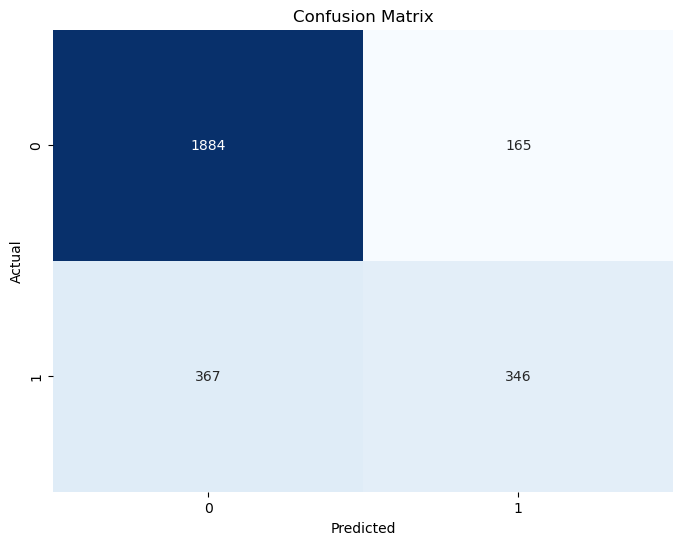
\includegraphics[width=0.8\textwidth]{confusion_matrix.png}
    \caption{Confusion Matrix of the Best Model}
    \label{fig:conf_matrix}
\end{figure}

\subsection{Discussion on the Suitability of Classification Models (Task 2.1)}

Each classification model employed had strengths relevant to detecting misinformation in social networks, particularly for Twitter's diverse and high-dimensional data. For instance:

\textbf{KNN:} KNN is effective for classifying social media profiles based on local patterns in the data, using distance metrics to identify bot-like behaviors (Zaki \& Meira, 2014).

\textbf{SVM:} The ability of SVM to handle high-dimensional data makes it suitable for Twitter datasets, which often include sparse text-based features. SVM’s robust performance in separating classes in complex spaces is crucial when identifying nuanced patterns in human vs. bot behavior (Cortes \& Vapnik, 1995).

\textbf{Decision Trees:} Decision Trees' intuitive structure and capability to work with mixed feature types, such as usernames and tweet content, make them useful, although prone to overfitting without proper tuning (Quinlan, 1986).

\textbf{Random Forest:} Random Forests' ensemble approach and robustness to noise make them ideal for handling the diversity of features in Twitter profiles, providing both high accuracy and interpretability through feature importance (Breiman, 2001).

\subsection{Comprehensive Evaluation for Stakeholders (Task 2.2)}

For stakeholders, such as social media platforms aiming to detect and mitigate the influence of bot accounts, Random Forest is recommended due to its high accuracy, robustness, and ability to generalize across various data types. Additionally, the model's ability to identify feature importance allows stakeholders to understand the key attributes of bot profiles, such as specific patterns in tweet frequency or profile setup. Decision Trees can also be useful in providing transparent, interpretable rules for non-technical stakeholders.

\subsection{Multi-Modality Approach (Task 2.3)}

Incorporating multiple modalities, such as profile colors, location, and tweet content, enhanced the classification models' ability to detect non-human profiles. Random Forest was particularly effective at integrating these diverse feature types, improving the model’s robustness across different data sources.

\subsection{Visualizations (Task 3)}

Key visualizations used to demonstrate model performance include:
\begin{itemize}
    \item Confusion matrices for each classification model.
    \item ROC curves to compare the performance of models like Random Forest and SVM, highlighting their ability to distinguish between human and bot profiles.
    \item Feature importance plots for Decision Trees and Random Forest to show which attributes (e.g., tweets, profile colors) contributed most to the classification.
\end{itemize}

\subsection{Result Summarization and Suggestions (Task 4)}

Random Forest emerged as the best-performing model for identifying non-human profiles, with high accuracy and robust performance across diverse features. Further improvements could be achieved by incorporating network-based features, such as retweet frequency or follower interactions, or by fine-tuning hyperparameters through more extensive cross-validation. These models provide valuable tools for stakeholders in the fight against misinformation on social media platforms, with potential applications in broader misinformation detection tasks (Ferrara et al., 2016).











\section{Task 3: Visualization}

\begin{figure}[h!]
    \centering
    \begin{minipage}{0.45\textwidth}
        \centering
        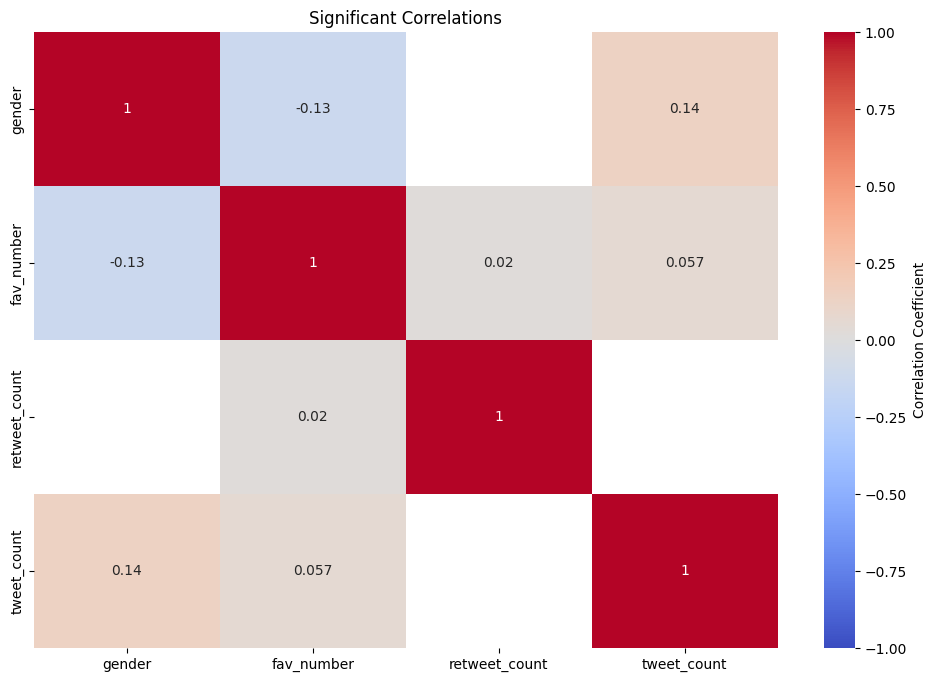
\includegraphics[width=\textwidth]{corr_a2.png}
        \caption{Correlation Matrix}
        \label{fig:corr}
    \end{minipage}
    \hfill
    \begin{minipage}{0.45\textwidth}
        \centering
        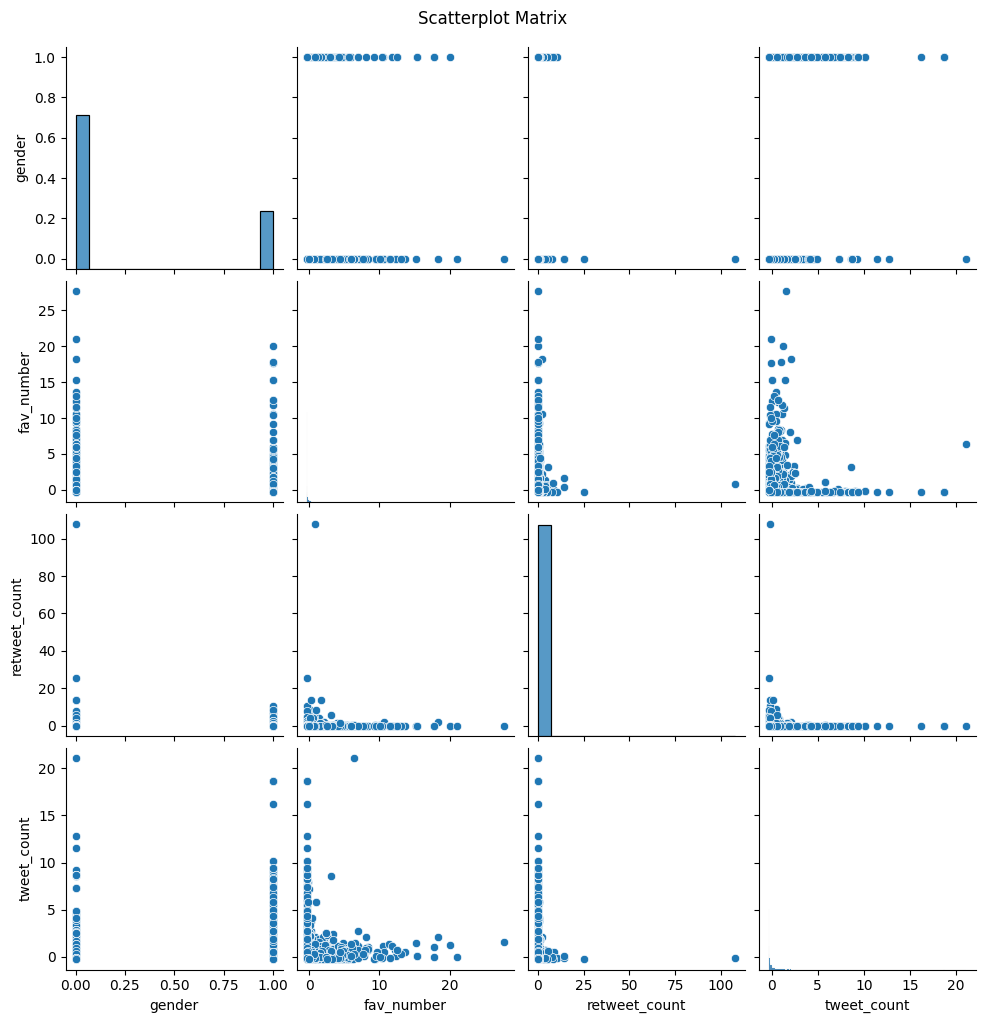
\includegraphics[width=\textwidth]{pair_plot_a2.png}
        \caption{Pair Plot}
        \label{fig:p_plot}
    \end{minipage}
\end{figure}

\begin{figure}[h!]
    \centering
    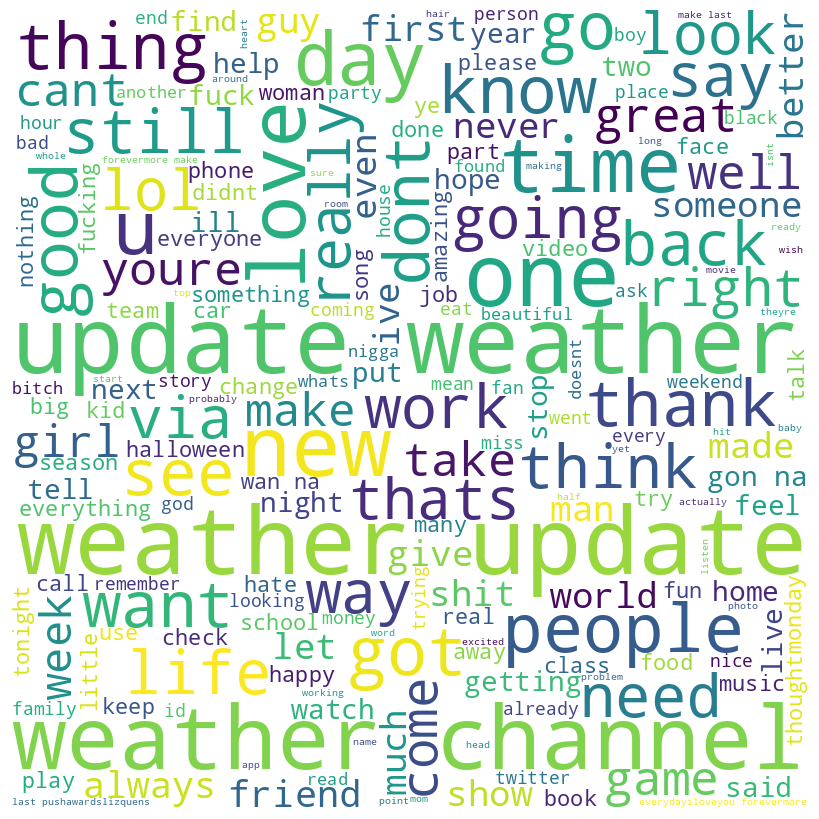
\includegraphics[width=0.5\textwidth]{word_cloud_a2.png}
    \caption{Word Cloud}
    \label{fig:wc}
\end{figure}

\begin{figure}[h!]
    \centering
    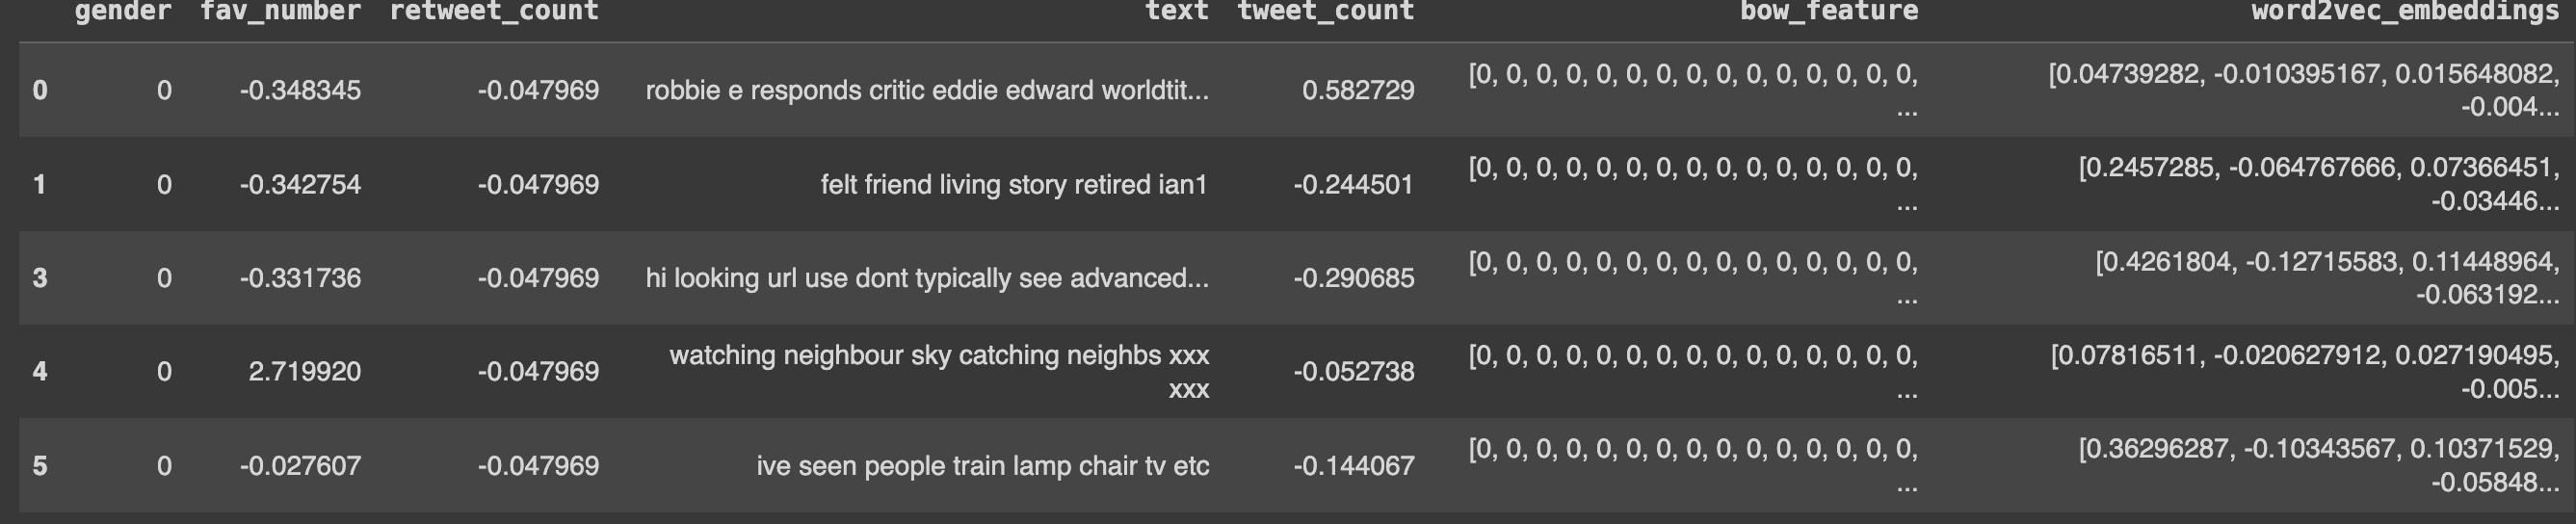
\includegraphics[width=0.5\textwidth]{df.png}
    \caption{Data Frame}
    \label{fig:df}
\end{figure}


\newpage
\bibliography{name}
\nocite{*}
\end{document}
